\documentclass[fleqn]{article}
\usepackage[margin=3cm]{geometry}   % shrink margins
\usepackage[margin=3cm]{caption}   % shrink captions
\usepackage{amsmath}    % math equation environments
\usepackage{amssymb}    % math symbols such as natural numbers N.
\usepackage{gensymb}	% general symbols such as \degree

\newenvironment{answers}{ % same as enumerate but with more space between each answer
	\begin{enumerate}
		\setlength{\itemsep}{\bigskipamount}
}{\end{enumerate}}

\newcommand\Item[1][]{ % custom \Item command for block math
  \ifx\relax#1\relax  \item \else \item[#1] \fi
  \abovedisplayskip=0pt\abovedisplayshortskip=0pt~\vspace*{-\baselineskip}}

\usepackage{multicol}	% can be used to put enumerate in columns. Usage: \begin{multicols}{NumCols}\begin{enumerate}...

\newcommand*{\perm}[2]{{}^{#1}\!P_{#2}}
\newcommand*{\comb}[2]{{}^{#1}C_{#2}}

\usepackage{tikz}	% for diagrams
% \usetikzlibrary{positioning}
% \usetikzlibrary{arrows}
% \usetikzlibrary{shapes}
% \usetikzlibrary{quotes}

\usepackage{pgfplots} % for plotting graphs
\pgfplotsset{
	/pgfplots/xlabel near ticks/.style={
		/pgfplots/every axis x label/.style={
        	at={(ticklabel cs:0.5)},anchor=near ticklabel
		}
	},
	/pgfplots/ylabel near ticks/.style={
		/pgfplots/every axis y label/.style={
			at={(ticklabel cs:0.5)},rotate=90,anchor=near ticklabel
		}
	}
}

% \usepackage{adjustbox}	% align enumerations containing tall objects to top. Usage: \item\adjustbox{valign=t}{...}

% \usepackage{centernot}	% centers not symbol. Usage: \centernot{...}

% Math mode in tables. Usage: use column type C
\usepackage{array}   % for \newcolumntype macro
\newcolumntype{C}{>{$}c<{$}} % math-mode version of "c" column type

% paragraph indentation within enumerations
\usepackage{enumitem}
\setlist{parsep=4pt,listparindent=\parindent}

\title{
	Statistics \\
	\medskip
	\large Homework 1 -- Representation of Data
}
\author{Abraham Murciano}

\begin{document}

\maketitle

\begin{answers}

	\item[1.]
	\begin{enumerate}
		\item % a
		For the following data set,
		\[1,8,1,5,8,6,3,3,3,7\]
		the mid-range, average, median and mode are as follows.
		\begin{align*}
			\text{Mid-range} &= \frac{1+8}{2} = 4.5 \\
			\text{Average} &= \frac{1+8+1+5+8+6+3+3+3+7}{10} = 4.5 \\
			\text{Median} &= \frac{3+5}{2} = 4 \\
			\text{Mode} &= 3
		\end{align*}

		\item % b
		For the following data set,
		\[14,18,30,31,15,18,27\]
		the mid-range, average, median and mode are as follows.
		\begin{align*}
			\text{Mid-range} &= \frac{14+31}{2} = 22.5 \\
			\text{Average} &= \frac{14+18+30+31+15+18+27}{7} \approx 21.86 \\
			\text{Median} &= 18 \\
			\text{Mode} &= 18
		\end{align*}
	\end{enumerate}

	\item[3.]
	In the month of August 2010 it was very hot. The Israeli meteorological service recorded the maximum temperature. The results are presented in Table \ref{q3-temperature}.
	\begin{table}
		\centering
		\begin{tabular}{||c|c||}
			\hline
			Number of days & Max. temperature (\degree C) \\
			\hline
			2	& 27-29 \\
			6	& 30-32 \\
			12	& 33-35 \\
			5	& 36-38 \\
			4	& 39-41 \\
			\hline
		\end{tabular}
		\caption{Maximum daily temperature frequencies for August 2010}
		\label{q3-temperature}
	\end{table}
	\begin{enumerate}
		\item % a
		Table \ref{q3-frequencies} shows the frequency, relative frequency, cumulative frequency, and relative cumulative frequency.
		\begin{table}[h]
			\centering
			\begin{tabular}{||c||c|c|c|c||}
				\hline
				Max. temp. (\degree C) & Frequency & Relative frq. & Cumulative frq. & relative cumulative frq. \\
				\hline
				27-29 & 2	& 0.0690 & 2	& 0.0690 \\
				30-32 & 6	& 0.2069 & 8	& 0.2759 \\
				33-35 & 12	& 0.4138 & 20	& 0.6897 \\
				36-38 & 5	& 0.1724 & 25	& 0.8621 \\
				39-41 & 4	& 0.1379 & 29	& 1.0000 \\
				\hline
			\end{tabular}
			\caption{Many types of frequencies of the data in Table \ref{q3-temperature}}
			\label{q3-frequencies}
		\end{table}

		\item % b
		Figure \ref{q3-bar-graphs} shows a bar graph of the data in Table \ref{q3-temperature} as well as a histogram.
		\begin{figure}[h]
			\centering
			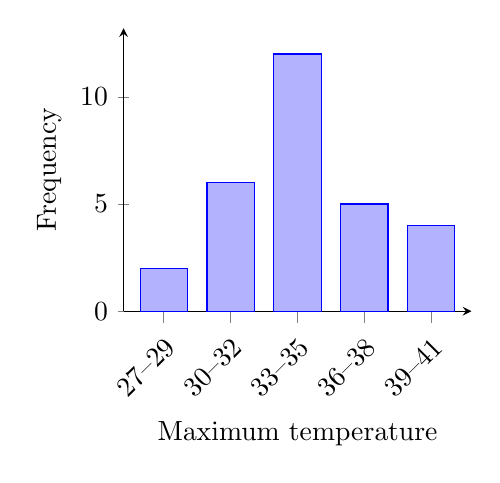
\begin{tikzpicture}
				\begin{axis}[
					width = 6cm,
					axis lines = left,
					xlabel = Maximum temperature,
					ylabel = Frequency,
					xlabel near ticks,
					ylabel near ticks,
					ymin = 0,
					enlarge x limits=0.15,
					enlarge y limits = {value=.1,upper},
					bar width = 0.6cm,
					ybar,
					symbolic x coords={27--29,30--32,33--35,36--38,39--41},
					x tick label style={rotate=45,anchor=north east},
					xtick = data
					]
					\addplot coordinates {(27--29,2) (30--32,6) (33--35,12) (36--38,5) (39--41,4)};
				\end{axis}
			\end{tikzpicture}
			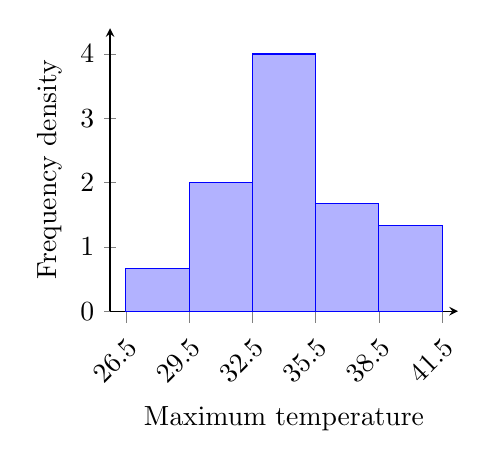
\begin{tikzpicture}
				\begin{axis}[
					width = 6cm,
					axis lines = left,
					xlabel = Maximum temperature,
					ylabel = Frequency density,
					xlabel near ticks,
					ylabel near ticks,
					ymin = 0,
					enlarge x limits=0.05,
					enlarge y limits = {value=.1,upper},
					ybar,
					symbolic x coords={26.5,29.5,32.5,35.5,38.5,41.5},
					x tick label style={rotate=45,anchor=north east},
					xtick = data
				]
					\addplot+[ybar interval] coordinates {(26.5,0.67) (29.5,2) (32.5,4) (35.5,1.67) (38.5,1.33) (41.5,0)};
				\end{axis}
			\end{tikzpicture}
			\caption{Bar graph of the data in Table \ref{q3-temperature} (left) and a histogram of the same (right)}
			\label{q3-bar-graphs}
		\end{figure}

		\item % c
		The mid-range, average, median and mode for this data are as follows.
		\begin{align*}
			\text{Mid-range} &= \frac{28 + 40}{2} = 34 \\
			\text{Average} &= \frac{2 \times 28 + 6 \times 31 + 12 \times 34 + 5 \times 37 + 4 \times 40}{29} \approx 34.3103 \\
			\text{Median} &= \frac{3 \left( \frac{29}{2} - 8 \right)}{12} + 32.5 = 34.125 \\
			\text{Modal class} &= [32.5,35.5)
		\end{align*}
	\end{enumerate}

	\item[6.]

\end{answers}

\end{document}
